
\documentclass{beamer}

\setbeamertemplate{frametitle}
 	{\begin{centering}\smallskip
    \insertframetitle\par
    \smallskip\end{centering}}
\setbeamertemplate{itemize item}{$\bullet$}
\setbeamertemplate{navigation symbols}{}
\setbeamertemplate{footline}[text line]{%
    \hfill\strut{%
	\scriptsize\sf\color{black!60}%
	\quad\insertframenumber
	}%
    \hfill
    }    
    % Define some colors:
    \definecolor{DarkFern}{HTML}{407428}
    \definecolor{DarkCharcoal}{HTML}{4D4944}
    \colorlet{Fern}{DarkFern!85!white}
    \colorlet{Charcoal}{DarkCharcoal!85!white}
    \colorlet{LightCharcoal}{Charcoal!50!white}
    \colorlet{AlertColor}{orange!80!black}
    \colorlet{DarkRed}{red!70!black}
    \colorlet{DarkBlue}{blue!70!black}
    \colorlet{DarkGreen}{green!70!black}
     
    % Use the colors:
    \setbeamercolor{title}{fg=Fern}
    \setbeamercolor{frametitle}{fg=Fern}
    \setbeamercolor{normal text}{fg=Charcoal}
    \setbeamercolor{block title}{fg=black,bg=Fern!25!white}
    \setbeamercolor{block body}{fg=black,bg=Fern!25!white}
    \setbeamercolor{alerted text}{fg=AlertColor}
    \setbeamercolor{itemize item}{fg=Charcoal}

  \usepackage[T1]{fontenc}
  \usepackage[utf8]{inputenc}
  \usepackage{lmodern}
  \usepackage[french]{babel}
    \usepackage{tikz}  
      \usepackage{pgfplots}
  \usepackage{mathabx}
  \usetikzlibrary{decorations.pathmorphing}
  \usetikzlibrary{decorations.pathreplacing}
  \usetikzlibrary{decorations.shapes}
  \usetikzlibrary{decorations.text}
  \usetikzlibrary{decorations.markings}
  \usetikzlibrary{decorations.footprints}
  
  
  
 
\DeclareMathOperator{\e}{e}
\def\Tr{\mathop{\rm{Tr}}\nolimits}
\def\bwp{{\bar \wp}}
\def\bwp{{\bar {\wp'}}}

\begin{document}
\title{Compter les points sur une courbe elliptique}   
\author{Jeremie Coulaud} 
\date{\today} 

\frame{\titlepage} 

\frame{\frametitle{Table of contents}\tableofcontents} 


\section{Introduction} 
\frame{\frametitle{Introduction} 

On définit une courbe elliptique sur un corps $K$ dans un plan par une équation de Weierstrass de la forme : 
\begin{equation*}
y^2 + a_1xy + a_3y  = x^3 + a_2x^2 + a_4x + a_6
\end{equation*}
Les coefficients $a_{1 \leq i \leq 6}$ sont des éléments du corps $K$.


Si  $car(K) \ne 2,3$ on se ramène à l'équation courte suivante : 
\begin{equation*}
y^2 = x^3 + ax +b
\end{equation*}
\begin{itemize}
\item $\Delta = -16(4a^3 + 27b^2) \quad \text{et} \quad j(E) = \frac{(-48a)^3}{\Delta}$
\item $E(K) = \left\{ (x,y) \in \mathbb{K} \, | \, y^2 = x^3 + ax + b = 0 \right\} \bigcup {O}$
\item $E[l] = \left\{ P \in E(\overline{\mathbb{K}}) \, | \, [l]P = 0 \right\} $
\end{itemize}
}

\section{Algorithme naïf}
\frame{\frametitle{Algorithme naïf}
$$ y^2 = x^3 +ax+b = f(x) $$
\begin{itemize}
\item  $\genfrac(){}{0}{f(x)}{p} = -1$, $f(x)$ n'est pas un carré modulo $p$, on ne trouve aucun point appartenant à la courbe.
\item $\genfrac(){}{0}{f(x)}{p} = 0$, $f(x)$ est divisible par $p$, on trouve $1$ point sur la courbe.
\item $\genfrac(){}{0}{f(x)}{p} = 1$, $f(x)$ est un carré modulo $p$, on trouve $2$ points sur la courbe.
\end{itemize}
}

\begin{frame}
\frametitle{}
\begin{equation*}
\#E(\mathbb{F}_p) = 1 + p +\sum_{x \in \mathbb{F}_p}\genfrac(){}{0}{f(x)}{p}
\end{equation*}
Complexité en la taille de $p$
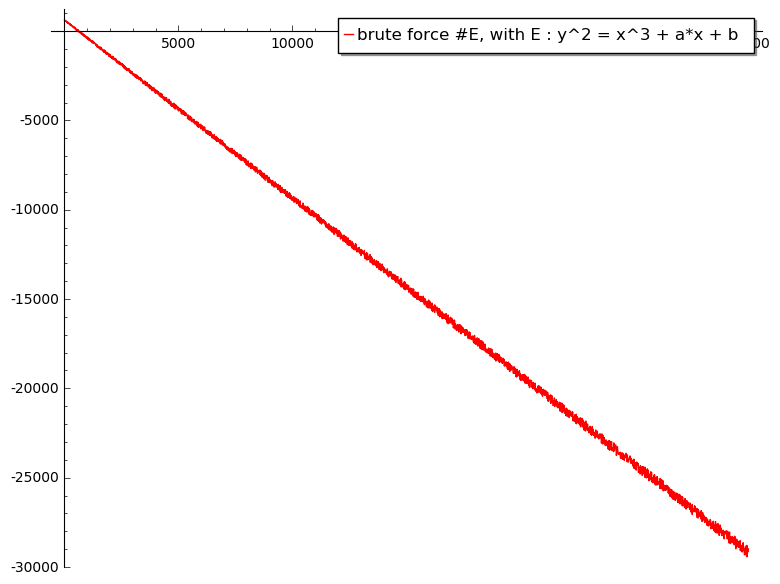
\includegraphics[scale=0.4]{../pictures/brute_force_cputime.png} 
\end{frame}

\section{Algorithme de Schoof}
\begin{frame}
\frametitle{Algorithme de Schoof}

\begin{block}{Théorème Hasse-Weil}
$\#E(\mathbb{F}_p) = p + 1 - t$ avec $|t| \leq 2 \sqrt{p}$ trace de l'endomorphisme de Frobenius de $E$.
\end{block}
Pour trouver l'ordre de $E(\mathbb{F}_p)$ il faut trouver $t$
\newline
Idée de Schoof : trouver $t \pmod l$, avec $l$ petit premier et utiliser les restes chinois pour trouver $t$
\end{frame}

\subsection{Frobenius}
\begin{frame}
\frametitle{Frobenius}
Soit $E$ une courbe elliptique défini sur $\mathbb{F}_p$, l'endomorphisme de Frobenius est défini par 

$\begin{array}{ccccc}
\phi_p & : & E(\mathbb{F}_p) & \to & E(\mathbb{F}_p) \\
 & & (x,y) & \mapsto & (x^p, y^p) \\
\end{array}$

On lui associe son polynôme caractéristique :
\begin{equation*}
\chi_p = \phi_p^2 - t \phi_p + p 
\end{equation*}
1ère application : calcul de $\#E(\mathbb{F}_{p^n})$
\begin{itemize}
\item $r_1,r_2$ racines de $\chi_p(x)$
\item $Tr(\phi_{p^n}(x,y)) = r_1^n + r_2^n$
\item Hass-Weil : $\#E(\mathbb{F}_{p^n}) = p^n +1 - r_1^n -r_2^n$
\end{itemize}
\end{frame}

\subsection{Polynômes de division}
\begin{frame}
\frametitle{Polynômes de division}
On appelle $f_n(X)$ le n-ième polynôme de division défini sur $\mathbb{Z}[x]$par : 
\begin{align*}
f_0(x) &= 0 \\
f_1(x) &= 1 \\
f_2(x) &= 1 \\
f_3(x) &= 3x^4 + 6ax^2 +12bx - a^2 \\
f_4(x) &= 2x^6 + 10ax^4 +40bx^3 - 10a^2x^2 - 8abx - 2(a^3 + 8b^2)
\end{align*}
On pose $F(X)= 4x^3 + 4ax + 4b$, et on a:

\begin{equation}
\left\lbrace
\begin{array}{ll}
f_{2n}& =  f_n(f_{n+2}f_{n-1}^2 - f_{n-2}f_{n+1}^2)   \\
f_{2n+1}& = \left\lbrace 
\begin{array}{ccc}
F^2f_{n+2}f_n^3 - f_{n-1}f_{n+1}^3 & \mbox{si} & n \text{ est pair}\\
f_{n+2}f_n^3 - f_{n-1}f_{n+1}^3F^2 & \mbox{si} & n \text{ est impair} \end{array}\right.

\end{array} \right.
\end{equation} 
\end{frame}

\begin{frame}
Ces polynômes s'annulent sur les points de $l$-torsion et permettent de calculer :

\begin{equation}\label{mP}
[m]P = \left\lbrace
\begin{array}{lll}
O_E & \mbox{si} & P \in E[m]  \\
\left(  x -   \frac{\psi_{m-1}(x,y)\psi_{m+1}(x,y)}{\psi^2_m(x,y)}, \frac{\psi_{2m}(x,y)}{\psi^4_m(x,y)}\right) & \mbox{sinon}  & 
\end{array}\right.
\end{equation}
En posant : 
\begin{equation*}
\psi_m= \left\lbrace
\begin{array}{cc}
2yf_m & \mbox{si m est pair} \\
f_m & \mbox{sinon}
\end{array}\right.
\end{equation*} 
\end{frame}


\begin{frame}
\frametitle{Frobenius et Schoof}
\begin{equation}
\label{eqnfrobenius}
\phi_p^2(P)  + [p_l]P = [t_{l}] \phi_p(P) \quad \forall P \in E[l]
\end{equation} 
Or pour tout $P=(x,y) \in E[l]$, $f_l(x) = 0$ et $y^2 - x^3 -ax -b=0$. 
\newline
On peut donc travailler dans l'anneau : 
$$ \frac{\mathbb{F}_p[x,y]}{(f_l(x), y^2 - x^3 -ax -b)} $$ 
La question est donc pour quelle valeur $0 \leq \tau \leq \frac{l-1}{2}$ l'équation suivante est vérifiée :
\begin{equation}
(x^{p^2}, y^{p^2}) + [p_l](x,y) = [\tau_l](x^{p}, y^{p})
\end{equation}
\end{frame}

\subsection{Choix des premiers $l$}
\begin{frame}
\frametitle{Choix des premiers $l$}
\begin{itemize}
\item $S = (l_1, \ldots l_n)$ tel que $\prod l_i > 4\sqrt{p}$
\item Petits $l_i$ pour que $f_l$ soit de plus petit degré possible.
\end{itemize}

 
\textbf{Cas} $\mathbf{l=2}$ \textbf{:} $t_2 \equiv 0 \pmod 2 \Leftrightarrow E(\mathbb{F}_p)$ a un élément d'ordre $2$
\begin{itemize}
\item Point $2$-torsion est de la forme $(x,0)$
\item $x^3 +ax +b$ a une racine dans $\mathbb{F}_p$
\item Calcul $\gcd(x^p - x,\, x^3 +ax +b) \ne 1$
\end{itemize}
\end{frame}

\subsection{Expérimentations}
\begin{frame}
\frametitle{Expérimentations}
\begin{columns}[T]
	\begin{column}{5cm}
		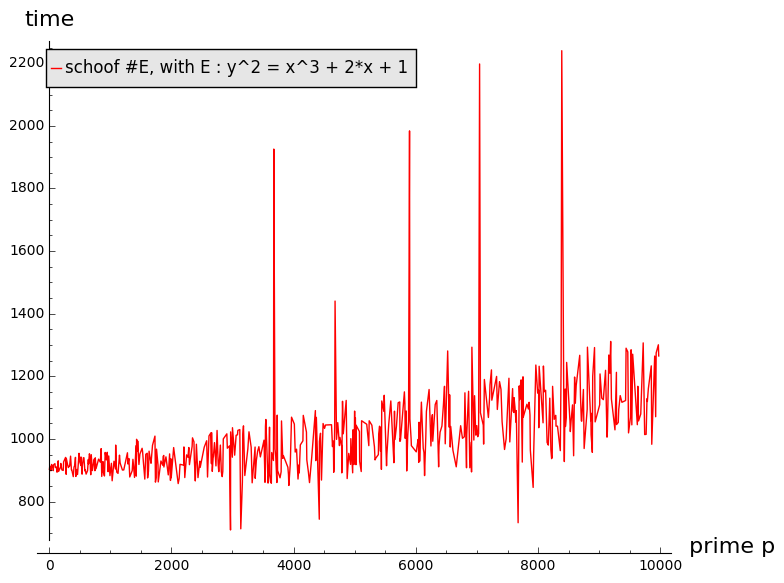
\includegraphics[scale=0.4]{../pictures/schoof_cputime.png} 
	\end{column}
	\begin{column}{5cm}
		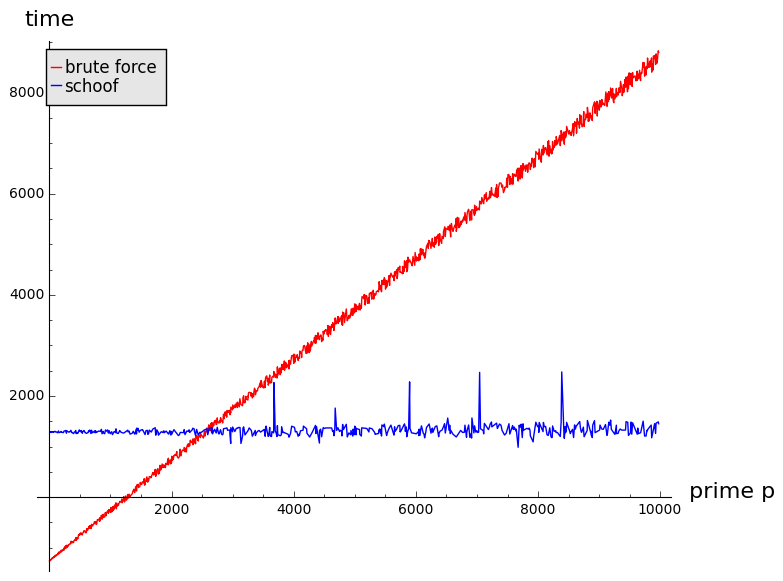
\includegraphics[scale=0.4]{../pictures/schoof_vs_bruteforce.png} 
	\end{column}
\end{columns}
\end{frame}

\section{Algorithme SEA}
\subsection{Analyse Complexe}
\begin{frame}
\frametitle{Analyse Complexe}
\begin{definition}
Tout sous groupe discret de $\mathbb{C}$ non nul et non isomorphe à $\mathbb{Z}$ peut s'écrire sous la forme $\mathbb{Z}\omega_1 + \mathbb{Z}\omega_2$, avec $\omega_1, \omega \in \mathbb{C}$, $Im(\frac{w_2}{w_1}) \ne 0, \tau = \frac{\omega_2}{\omega_1}$. C'est un réseau de $\mathbb{C}$ de rang $2$, qu'on note :
$$\Gamma = \mathbb{Z} + \tau \mathbb{Z}$$
\end{definition}

\begin{definition}
On appelle tore le quotient $T=\mathbb{C} / \Gamma$
\end{definition}
\end{frame}

\begin{frame}
Soit $\Gamma$ un réseau de $\mathbb{C}$, on a la $\wp$-fonction de Weirstrass :
$$ \wp(z) = \frac{1}{z^2} + \sum_{w \in \Gamma, \omega \ne 0} \frac{1}{(z-\omega)^2} - \frac{1}{\omega^2} $$
et sa dérivée : 
$$ {\wp'} = -2 \sum_{\omega \in \Gamma} \frac{1}{(z-\omega)^3} $$
\begin{theorem}
Soit $E$/$\mathbb{C}$ une courbe elliptique sous forme réduite sur le corps des complexes. Il existe alors un réseau $\Gamma$ tel que l'application suivante soit une bijection:
\newline
$\begin{array}{cccc}
& \mathbb{C}\text{/ }\Gamma & \to & E \\
& z + \Gamma & \mapsto & \left\lbrace
\begin{array}{cc}
 (\wp(z), \frac{{\wp'}(z)}{2})  & z \notin \Gamma \\
 O & z \in \Gamma
\end{array}\right.\\
\end{array}$
\end{theorem}
La fonction $\wp$ satisfait l'équation différentielle suivante : 
\begin{equation*}
{\wp'}(z)^2 = 4\wp^3(z) + A \wp + B
\end{equation*}
\end{frame}


\subsection{Isogénie}
\begin{frame}
\frametitle{Isogénie}
\begin{definition}
Soit $E_1$/$K$ et $E_2$/$K$ deux courbes elliptiques. Si $E_1$ et $E_2$ ont le même $j$-invariant alors elles sont isomorphiques sur $\bar{K}$. 
\end{definition}

\begin{definition}
Soit $T_1=\mathbb{C}$/ $\Gamma_1$ et $T_2 = \mathbb{C}$/ $\Gamma_2$ deux tores. Un morphisme de $E_1$ vers $E_2$ est une application holomorphe $\mu$ de $T_1$ vers $T_2$ qui soit un morphisme de groupe. Si ce morphisme est non constant alors on dit que c'est une isogénie.
\end{definition}

Deux courbes elliptiques $E_1$/$K$ et $E_2$/$K$ sont isogènes s'il existe une isogénie $\psi : E_1 \mapsto E_2$. Le degré de l’isogénie est le degré du noyau de $\psi$.


\end{frame}
\subsection{Polynômes modulaires}
\begin{frame}
\frametitle{Polynômes modulaires}
Le $n$-ème polynome modulaire est noté $\Phi_n(X,Y)$ et il est :
\begin{itemize}
\item symétrique 
\item de degré $n+1$ en chaque variable
\item de coefficients de termes de plus haut degré $1$
\item de coefficients dans $\mathbb{Z}$
\end{itemize}
\begin{definition}
Soit $E_1$/$\mathbb{C}$ et $E_2$/$\mathbb{C}$ deux courbes elliptiques de $j$-invariant respectivement $j_{E_1}$ et $j_{E_2}$. Le $n$-ième polynôme modulaire vérifie $\Phi_n(j_{E_1},j_{E_2}) = 0$ si et seulement si il existe une isogénie entre $E_1$ et $E_2$ dont le noyau est cyclique de degré $n$.
\end{definition}


\end{frame}

\begin{frame}
\begin{example}
Pour $n=3$ on a le polynôme : 
\begin{align*}
\Phi_3(x,y) &= x^4 -x^3y^3 + y^4 \\
 +& 2232(x^3y^2 + x^2y^3) \\
 -& 1069956(x^3y^2 + x^2y^3 \\
 +& 36864000(x^3 + y^3) \\
 +& 2587918086x^2y^2 \\
 +& 8900222976000(x^2y + xy^2) \\
 +& 452984832000000(x^2 + y^2) \\
 -& 770845966336000000xy \\
 +& 1855000000000(x+y) 
\end{align*}
\end{example}
\end{frame}

\begin{frame}
\frametitle{Algorithme SEA}
Amélioration de l'algorithme de Schoof par Elkies et Atkins.
\bigskip
\begin{columns}[T]
	\begin{column}{5cm}
		\begin{tikzpicture}[scale = 0.7]
\begin{axis}[
  axis x line=center,
  axis y line=center,
  title = {Représentation de $E[6]$},
  xtick={0,...,5},
  ytick={0,...,5},
  xticklabels={$0$,$P_1$, $2P_1$, $3p_1$, $4P_1$, $5P_1$},
  yticklabels={$0$,$P_2$, $2P_2$, $3p_2$, $4P_2$, $5P_2$},
  xmin=0,
  xmax=5.5,
  ymin=0,
  ymax=5.5]
\addplot[only marks] coordinates {
(0,0) (0,1) (0,2) (0,3) (0,4) (0,5) (1,0) (2,0) (3,0) (4,0) (5,0) (1,1) (2,2) (3,3) (4,4) (5,5) (1,2) (1,3) (1,4) (1,5) (2,1) (2,3) (2,4) (2,5) (3,1) (3,2) (3,4) (3,5) (4,1) (4,2)
(4,3) (4,5) (5,1) (5,2) (5,3) (5,4) 
};
\end{axis}
\end{tikzpicture}
	\end{column}
	\begin{column}{5cm}
		 \begin{tikzpicture}[scale = 0.7]

\begin{axis}[
  axis x line=center,
  axis y line=center,
  title = {Représentation d'un sous groupe de $E[6]$},
  xtick={0,...,5},
  ytick={0,...,5},
  xticklabels={$0$,$P_1$, $2P_1$, $3p_1$, $4P_1$, $5P_1$},
  yticklabels={$0$,$P_2$, $2P_2$, $3p_2$, $4P_2$, $5P_2$},
  xmin=0,
  xmax=5.5,
  ymin=0,
  ymax=5.5]
\addplot[only marks] coordinates {
(0,0) (1,1) (2,2) (3,3) (4,4) (5,5) 
};
\end{axis}
\end{tikzpicture}
	\end{column}

\end{columns}
\end{frame}

\begin{frame}
Soit $l$ un petit premier, $\phi$ l'endomorphisme de Frobenius de polynôme caractéristique :
$$\chi_l(x) = x^2 - t_lx +p_l, \quad \text{avec } t \equiv t_l \pmod l , \, \,p \equiv p_l \pmod l$$ 
\newline 
$$\Delta_{\chi_l} = t_l^2 -4p_l $$
\begin{definition}
Si $\Delta_{\chi_l}$ est un carré non nul dans $\mathbb{F}_l$, alors $l$ est un premier de Elkies, sinon c'est un premier de Atkins.
\end{definition}
Étude de la factorisation de $\Phi_l$ pour savoir si $\Delta_{\chi_l}$ est un carré. 
\newline
$\Phi_l(x,j) = h_1(x)\ldots h_s(x)$:
\begin{itemize}
\item $(1,1,r,\ldots,r)$, $\Delta_{\chi_l}$ est un carré, $\phi_{|E[l]}$ est diagonalisable, $l$ est un premier de Elkies
\item Calcul $\gcd(\Phi_l(x,j), x^p - x)$
\end{itemize}
\end{frame}
\subsection{Premier d'Elkies}
\begin{frame}
\frametitle{Premier d'Elkies}
\textbf{Premier d'Elkies}
\newline
$\phi_p$ est diagonalisable de valeurs propres $\lambda, \mu$. 
$$\chi_l(x) = x^2 - t_lx +p_l =(x-\lambda)(x-\mu)$$
Donc :
\begin{align*}
t_l &\equiv \lambda + \mu \pmod l
\end{align*}
\begin{itemize}
\item $\exists P_1 \in E[l]$ tel que $\phi_l(P_1) = \lambda P_1$
\item $C_1$ est le groupe cyclique d'ordre $l$ engendré par $P$
\item $C_1$ est stable par le Frobenius 
\end{itemize}
On peut construire le polynome de degré $l$ :
$$ g_l(x) = \prod_{\pm P \in C_1^*} (x - x_p), \quad \text{où } P = (x_p, y_p) $$
\end{frame}
\end{document}


